\chapter{Swarm movement metric}\label{chapter:metric}
%\section{Introduction\label{methods:SwarmStability}}
This chapter examines the distance metric as a mechanism to measure the internal movement of agents and introduces a new \textit{magnitude based metric}. The internal movement of a swarm is identified by analysing the changes in the inter-agent interactions. The two metrics differ in their approach to identifying the changes. The distance metric uses variations in the inter-agent spaces, as used by Navarro et al.~\cite{NIM:09}. The new metric, devised as part of this thesis, uses the magnitudes from the agents' \textit{inter-agent vectors} that are induced by agents' field effects as defined in~\autoref{eq:BotDirection3}. 

Both metrics allow a comparison of the effects of different swarming algorithms on a swarm's structure. The type of information that can be derived from each of the metrics is compared in~\autoref{metric:MagnitudeDistanceComparison}.

The magnitude based metric is used in chapter~\ref{chapter:coordination} to identify the effects of different coordination algorithms. In chapter~\ref{chapter:ConcaveReduction} the metric is used to identify the effects of both obstacles on a swarm's movement and the encapsulating behaviour a swarm exhibits when using \textit{concave reduction}.
 
%% \section{Metric principles\label{section:MagnitudeDynamics}}
%% This section discusses the theory behind swarm movement and the effects that can be measured using both the metrics described above.

\section{Inter-agent vector magnitude effect on internal movement}\label{Section:StabilityMagnitude}
\autoref{methods:Stability5} shows the cohesion and repulsion vector contributions to $v_c(b)$, $v_r(b)$ due to neighbour $b'$, as given in equations~\ref{eq:FlyToCentre1} and~\ref{eq:Repulsion1}. Notice that the vectors are along the line of separation $bb'$. 

Using the cohesion and repulsion vectors generated by the relationship of $b'$ to $b$ a resultant vector can be calculated. This vector creates an agent characteristic that can be used as a metric. Summing the vectors creates a resultant vector with a magnitude that affects the agent. Summing the vectors also provides an indication of the direction an agent will move based on the relationship. This is defined in chapter~\ref{chapter:methods} as the \textit{inter-agent vector}.

From here throughout \autoref{metric:MagnitudeDynamics2} and \autoref{metric:StabilityNullVector} imagine agent $b$ has just a single neighbour $b'$ and consider the effect of $b'$ on $v(b)$, the \textit{inter-agent vector} of $b$.
%% The relationship between the agents is that: \emph{the vector for $b$ with respect to $b^{'}$, and the vector for $b^{'}$ with respect to $b$ are on the same line}~(\autoref{methods:Stability5}).
%% If we consider an agent ($b$) as having only one neighbour ($b'$) then using the formulae defined in chapter~\ref{chapter:methods} the vectors $v_c(b)$~(\autoref{eq:FlyToCentre1}) and $v_r(b)$~(\autoref{eq:Repulsion1}) are the magnitudes of the vectors that are generated by the field effects between the two agents. $k_c$ and $k_r$ are the weighting factors for the cohesion and repulsion. The resulting vectors are aligned along the same line of separation between the agents. 

\begin{figure}[H]
\begin{center}
\includegraphics[width=7cm]{CHAPTER-4/figures/Stability5}
\end{center}
\caption{Vectors on line of separation} \label{methods:Stability5}
\end{figure}

\section{Swarm movement analysis\label{metric:MagnitudeDynamics2}}
The repulsive and cohesive vectors are generated for an agent through the intersection of their field effects~(\autoref{sec:Cohesion1} and~\autoref{sec:Repulsion1}). There are a limited number of intersections that can occur; These are illustrated in Figures~\ref{methods:Stability1}, \ref{methods:Stability2}, \ref{methods:Stability3},  and \ref{methods:Stability4}.

Figures~\ref{methods:Stability1}, \ref{methods:Stability2}, \ref{methods:Stability3}, \ref{methods:Stability4} show the cohesion of an agent pair as $k_cv_c$ and the repulsion as $k_rv_r$. The example data extracts~(Tables \ref{tab:SampleReplusion0}, \ref{tab:SampleReplusionPositive}, \ref{tab:SampleCohesionPositive}, \ref{tab:SampleEquilibrium}) are generated from the simulator using the parameters in table~\ref{tab:MetricPhysics1} that create a basic swarming behaviour. The tables show the simulation results. The simulation consists of 200 agents over a 20 second period. The simulation produces a neighbour extract of 248,798 records.

\begin{table}[H]
\begin{center}
\begin{tabular}{| p{2.5cm} | c | p{7cm} |}
\hline
\bf Weight \bf Component & \bf Swarm & \bf Description \\ \hline
Sample Rate & 100 & ms - Unit sampling interval\\  \hline
$k_c$ & 5 & weight adjuster for cohesion bias\\  \hline
$k_r$ & 15 & weight adjuster for repulsion  bias\\  \hline
$k_d$ & 0 & weight adjuster for directional bias 0 for static baseline 100 from directional\\  \hline
Repulsion field & 70 & units\\  \hline
Cohesion field & 80 & units\\  \hline
Speed & 20 & units/s\\  \hline
\end{tabular}\caption{Swarm parameters model} \label{tab:MetricPhysics1}
\end{center}
\end{table}

\autoref{methods:Stability1} shows two agents within each others cohesion fields but sufficiently distant to be outside of the repulsion fields. The `neighbour region' and `repulsion region' are the limits of the field effects for cohesion and repulsion. In this case $k_cv_c > 0$ and $k_rv_r = 0$: the result is the agent's resultant magnitudes cause the agents to move towards each other. \autoref{tab:SampleReplusion0} shows the repulsion magnitude with a value of 0. The only influence on the agent pairs are cohesive vectors. 

\begin{figure}[H]
\begin{center}
\includegraphics[width=11cm]{CHAPTER-4/figures/Stability1}
\end{center}
\caption{Internal movement cohesion (no repulsion)} \label{methods:Stability1}
\end{figure}

In tables~\ref{tab:SampleReplusion0},~\ref{tab:SampleReplusionPositive},~\ref{tab:SampleCohesionPositive}~and~\ref{tab:SampleEquilibrium}, \textbf{Log} is the sample identifier, \textbf{Id} is the unique identifier for an agent and \textbf{N.Id} is the Id of the agent neighbour. 

\begin{table}[H]
\begin{center}
\begin{tabular}{| l | l | l | l | l | l |}
\hline
Log &	Id &	N.Id &	Distance &	{\color{green}Cohesion} &	{\color{red}Repulsion} 	\\ \hline
0 &	1 &	3 	 & 70.50359957272653 &	{\color{green}352.5179978636327}  &	{\color{red}0} \\ \hline
0 &	1 &	100 & 71.78005530038806 &	{\color{green}358.9002765019403}  &	{\color{red}0} \\ \hline
0 &	1 &	151 & 78.33995887998715 &	{\color{green}391.69979439993574} &	{\color{red}0} \\ \hline
0 &	2 &	99  &	72.04066804327307 &	{\color{green}360.20334021636535} &	{\color{red}0} \\ 
\hline
\end{tabular}\caption{Data extract ($k_rv_r = 0$)} \label{tab:SampleReplusion0}
\end{center}
\end{table}

\autoref{methods:Stability2} shows two agents close together with repulsion dominating cohesion such that $k_cv_c < k_rv_r$. The resultant vector will direct the agents away from each other. \autoref{tab:SampleReplusionPositive} shows the repulsion magnitude with a value greater than cohesion.

\begin{figure}[H]
\begin{center}
\includegraphics[width=6.5cm]{CHAPTER-4/figures/Stability2}
\end{center}
\caption{Internal movement repulsion} \label{methods:Stability2}
\end{figure}

\begin{table}[H]
\begin{center}
\begin{tabular}{| l | l | l | l | l | l |}
\hline
Log &	Id &	N.Id &	Distance &	{\color{green}Cohesion} &	{\color{red}Repulsion} 	\\ \hline
0 & 1 &	2 &	28.325225929649267 &	{\color{green}141.62612964824635} &	{\color{red}1544.860149837827} \\ \hline
0 & 1 &	6 &	41.48517221724064  &	{\color{green}207.42586108620318} &	{\color{red}721.7173648240145} \\ \hline
0 & 1 &	7 &	35.264128136470426 & {\color{green}176.32064068235212} &	{\color{red}1034.271010913942} \\ \hline
0 & 1 &	8 &	43.545037655009644 &	{\color{green}217.72518827504823} &	{\color{red}637.9075999959364} \\
\hline
\end{tabular}\caption{Data extract ($|k_cv_c| < |k_rv_r|$)} \label{tab:SampleReplusionPositive}
\end{center}
\end{table}

\autoref{methods:Stability3} shows two agents close together but with cohesion vector magnitudes greater than the repulsion magnitudes $|k_cv_c| > |k_rv_r|$. The resultant vector will draw the agents together. The magnitude of the resultant cohesion vector will be reduced due to the cancelling effect of the repulsion vector. \autoref{tab:SampleCohesionPositive} shows a data extract with the cohesion magnitude greater than repulsion.

\begin{figure}[H]
\begin{center}
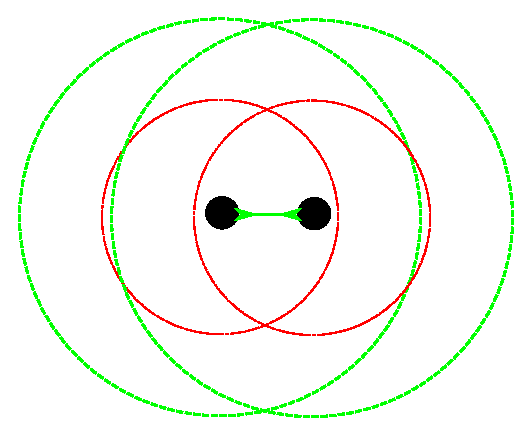
\includegraphics[width=6.5cm]{CHAPTER-4/figures/Stability3}
\end{center}
\caption{Internal movement cohesion} \label{methods:Stability3}
\end{figure}

\begin{table}[H]
\begin{center}
\begin{tabular}{| l | l | l | l | l | l |}
\hline
Log &	Id &	N.Id &	Distance &	{\color{green}Cohesion} &	{\color{red}Repulsion} 	\\ \hline
0 &	1 &	5 &	64.17214469587854 &	{\color{green}320.86072347939273} & 	{\color{red}95.35676418993891} \\ \hline
0 &	1 &	9 &	63.880497718571355 &	{\color{green}319.4024885928568} &	{\color{red}100.58590062663305} \\ \hline
0 &	1 &	95 &	65.6152270119206 &	{\color{green}328.07613505960296} & 	{\color{red}70.16681717258929} \\ \hline
0 &	1 &	152 &	63.10700566424517 &	{\color{green}315.53502832122587} & 	{\color{red}114.68844031437281} \\ 
\hline
\end{tabular}\caption{Data extract ($|k_cv_c| > |k_rv_r|$)} \label{tab:SampleCohesionPositive}
\end{center}
\end{table}

\autoref{methods:Stability4} shows two agents close together with $|k_cv_c| = |k_rv_r|$ the resultant vector will be a \textit{null vector} and the agents will have no influence upon each other due to the magnitude of the resultant vector being zero. \autoref{tab:SampleEquilibrium} is an extract from the \textbf{\texttt{NEIGHBOURS}} table. The data shows an extract that is near equilibrium. The simulation produced no null magnitude results. 

\begin{figure}[H]
\begin{center}
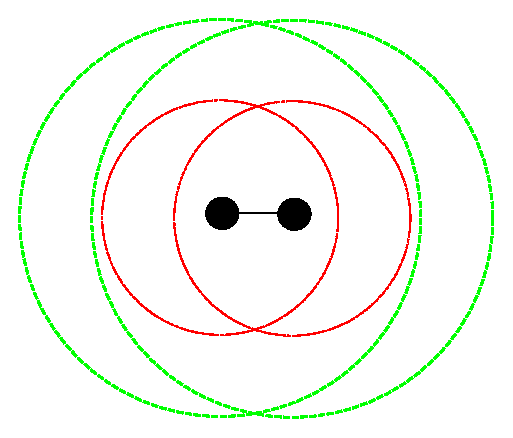
\includegraphics[width=6.5cm]{CHAPTER-4/figures/Stability4}
\end{center}
\caption{Internal movement equilibrium} \label{methods:Stability4}
\end{figure}

\begin{table}[H]
\begin{center}
\begin{tabular}{| l | l | l | l | l | l |}
\hline
Log &	Id &	N.Id &	Distance &	{\color{green}Cohesion} &	{\color{red}Repulsion} 	\\ \hline
7 &	76 &	91 &	55.390312278311875 &	{\color{green}276.9515613915594} &	{\color{red}276.9468428106153} \\ \hline
24 &	75 &	6 &	55.39032191143417 &	{\color{green}276.95160955717085} &	{\color{red}276.9466120367043} \\ \hline
32 &	72 &	38 &	55.39002603773678 &	{\color{green}276.9501301886839} &	{\color{red}276.95370011064875} \\ \hline
35 &	63 &	64 & 	55.390227283173054 &	{\color{green}276.9511364158653} &	{\color{red}276.9488789826377} \\
\hline
\end{tabular}\caption{Data extract ($|k_cv_c| \approx |k_rv_r|$)} \label{tab:SampleEquilibrium}
\end{center}
\end{table}

\section{Internal movement and the null vector}\label{metric:StabilityNullVector}
When the two vectors (cohesion and repulsion) have magnitudes that are equal and opposite they produce a null vector. This indicates that two agents are optimally spaced for a given set of conditions. Although the agents are at an optimum position it does not mean the swarm is optimally distributed. If a swarm is in a confined space it is possible for an optimum position to be created where the vector magnitude is positive due to a compression effect. This phenomenon is used in the identification of the emergent behaviour of area flooding, covered in chapter~\ref{chapter:flooding}.  

If we consider the equilibrium state (\autoref{methods:Stability4}) the resultant vector of $b$ is $(0,0)$. A null vector cannot be normalised to produce a directional vector ($\hat{v} = \frac{v}{|v|}$ if $v\neq0$; $0$ if $v=0$). The effect of the resultant magnitude being a null vector is that the agent will remain stationary. If all agent pairs are in this condition the swarm will stop moving~(\autoref{methods:StabilityNullVector}).

\begin{figure}[H]
\begin{center}
\includegraphics[width=7cm]{CHAPTER-4/figures/StabilityNullVector}
\end{center}
\caption{Equilibrium with null vectors} \label{methods:StabilityNullVector}
\end{figure}

Due to the independent nature of the agents this situation is very rare. The residual motion that persists in a swarm is the background `noise' or `jitter' that an algorithm creates.

If a swarm is goal-based the additional \textit{directional vector} will prevent all agents simultaneously producing null vectors~(\autoref{methods:StabilityNullVector2}).

\begin{figure}[H]
\centering
\subfigure[($t$)]{
	 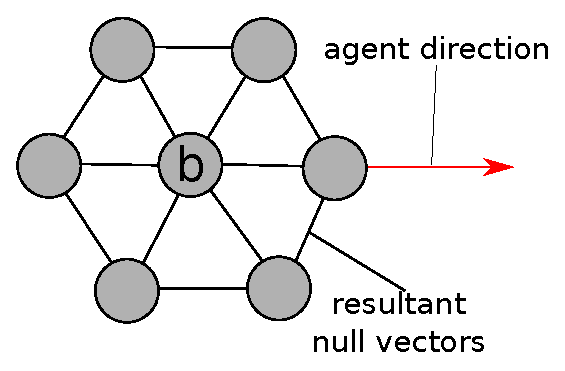
\includegraphics[width=5.5cm]{CHAPTER-4/figures/StabilityNullVector3}
    \label{metric:VoidPerimeter1}
}
\subfigure[($t + 1$)]{
	 \includegraphics[width=6cm]{CHAPTER-4/figures/StabilityNullVector2}
    \label{metric:VoidPerimeter2}
}
\caption{Directional movement and the null vector}
\label{methods:StabilityNullVector2}
\end{figure}

\section{Residual internal movement (Jitter)}\label{metric:Jitter}
Due to the dynamic nature of a swarm maintaining optimum internal movement as in~(\autoref{methods:Stability4}) a stationary swarm is highly unlikely. The agent pairs will fluctuate between the 3 states~(Figures~\ref{methods:Stability2}, \ref{methods:Stability3}, \ref{methods:Stability4}). This alternation between the states is \textit{jitter}. The degree to which this variation occurs can be measured using either the change in distance between the agent pairs, or the change in the resultant magnitude between the agent pairs. Jitter is motion that is produced to maintain the structure of a swarm. A coordination algorithm that produces minimal jitter is generally more desirable. Jitter (the fluctuation in and between the states) is an indication of the efficiency of an algorithm and an integral component of a swarm's measurable behaviour.

\section{Magnitude based metric\label{section:MagnitudeDynamics}}
Magnitude based internal movement (\textit{agent resultant magnitude}) is measured by identifying the balance between the repulsion and cohesion between agents. `Jitter' in the case of the \textit{agent resultant magnitude} metric is measured as the variance of the potentials created by the agents. The identification of this variance produces the clarifying part of the \textit{agent resultant magnitude} metric.
%% The magnitude based metric identifies the resultant internal magnitude (vector magnitude) through the cohesive and repulsive magnitudes that exist between each agent pair in a swarm. 
The \textit{agent resultant magnitude} is identified by Gazi and Passino~\cite{GP:11} and Barnes et al~\cite{BFV:07} as a `resultant characteristic' of a swarm. There are two ways of using the cohesion and repulsion in identifying a resultant vector. The two vectors can be added as absolute values to give an overall `size' to the magnitude that is affecting each relationship. Alternatively the resultant magnitude can be the sum of the actual magnitudes. The repulsion vector has a negative magnitude and the cohesion vector has a positive magnitude. In this thesis the magnitude analysis will be based on summing the two actual vectors to determine the result of the inter-agent interaction. This thesis will refer to the resultant magnitude as the \text{`agent resultant magnitude'} of the relationship. The `state' of a swarm is the effect the environmental constraints and algorithms have upon the agent resultant magnitude. It is a part of the `quality' measure for a swarm's performance.

If the \textit{agent resultant magnitude} is a negative value (absolute values would prevent this analysis) the swarm's bias is to expand. This is seen in the disorganised stage of a swarm. If the \textit{agent resultant magnitude} is positive then the swarm is exhibiting a tendency to contract and this indicates the swarm is a cohesive entity. This could also be described as the swarm being `sticky' as the agents bias is to `pull' towards each other.

The \textit{agent resultant magnitude} on its own does not give a complete measure of a swarm's internal state. There needs to be a qualifying component to the metric  that identifies the degree of deviation in the resultant magnitude, this is the \textit{jitter}. The smaller the degree of deviation the more uniform the structure of the swarm. These two components identify the degree to which a swarm has progressed towards a stable state. 

The \textit{agent resultant magnitude} provides a view of the swarm's state through the balance between the repulsive and the cohesive vectors that are being applied to each agent. The variance component identifies the degree to which the swarm has stabilised. The ideal status for inter-agent interactions would be for the agents to have a resultant vector (\textit{agent resultant magnitude}) of zero or above. This would indicate that the agents are distributed such that they are at their distribution limit (outer most range of the cohesion field) or at a level that causes the agents to `pull' together. The ideal degree of deviation is zero as this indicates an even distribution of agents. Therefore for a fuller indication of a swarm's \textit{state} both measurements need to be combined. The deviation from the mean clarifying the internal movement and the \textit{agent resultant magnitude} providing an indication of the `compression' that a swarm is logically experiencing (cohesiveness). These two aspects of a swarm's features are not considered by Gazi and Passino~\cite{GP:11} or Barnes et al~\cite{BFV:07} as a means of quantifying the structure of a swarm in terms of stability.

\section{Distance based metric\label{section:DistanceDynamics}}
The distance based metric considers the effect of the resultant vectors upon a swarm in terms of how the agents are physically distributed: i.e. only the inter-agent distances and the deviation from the mean of the agents (jitter) are considered. As with the \textit{agent resultant magnitude} metric the variations are important to determine the agent distribution. The standard deviation from the mean allows the internal `characteristic' of the measure to be realised. If the standard deviation is zero then all the agents are evenly spaced. The distance metric does not take into consideration the vector magnitudes between the agents as discussed above. The metric therefore is unable to identify the potential state of the swarm in terms of its cohesive or repulsive state.

Navarro and Fernando describe a mean distance error metric that is based on the variations in distances between inter-agent spaces~\cite{NIM:09}. This is the same as the standard deviation of the distance based internal movement metric as described here. 

\section{Magnitude based internal movement model}\label{Section:StabilityModel}
Using the formulae for the calculation of cohesion~(\autoref{eq:FlyToCentre1}, page \pageref{eq:FlyToCentre1}) and repulsion~(\autoref{eq:Repulsion1}, page \pageref{eq:Repulsion1}) for every agent and its neighbours it is possible to calculate an \textit{agent resultant magnitude} value (sum of agent resultant magnitudes). This value represents the overall potential of an agent. This magnitude when normalised produces a component of the \textit{movement-destination vector}~(\autoref{eq:BotDirection1}) for a swarm. If the agent resultant magnitude is zero (null vector) then the agent will not move. $P(b)$ is the \textit{inter-agent resultant magnitude vector} for agent $b$ defined by:

\begin{equation}
\label{eq:BotStabilityT}
P(b) = k_cv_c(b) + k_r v_r(b)
\end{equation}

Although it is possible for agent $b$ to have a resultant vector of null there could still be a variation in the constituent components. The variation calculation (standard deviation) is shown in~\autoref{Section:VarianceInPotential}. \autoref{eq:SwarmStabilityMetricT} is the mean of the \textit{agent resultant magnitudes} for an agent and its neighbours where $\card{nbr(b)}$ is the number of neighbours.

\begin{equation}
\label{eq:SwarmStabilityMetricT}
\mu_p(b) = \frac{P(b)}{\card{nbr(b)}}
\end{equation}

%% \autoref{eq:SwarmStabilityMetricT} should be considered as being applied at discrete points in time within a simulation. The formulae could also be shown based on time $t$ (\autoref{eq:SwarmStabilityMetricT2}) where $b_t$ is an agent at a specific time interval. All formulae for agent resultant magnitude in this thesis will be considered as being applied at a point in time and will therefore be shown without a $t$ subscript.
%% 
%% \begin{equation}
%% \label{eq:SwarmStabilityMetricT2}
%% \mu_p(b_{t}) = \frac{P(b_{t})}{|nbr(b_{t})|}
%% \end{equation}

To identify the swarm based \textit{agent resultant magnitude}~\autoref{eq:SwarmStabilityMetricT} must be extended to iterate over all the agents in the swarm. \autoref{eq:SwarmStabilityMetricT3} shows $\mu_p(S)$~as the swarm based magnitude where the swarm iteration is shown as~$\sum_{b \in S}$ and $\sum_{b \in S}\card{nbr(b)}$ calculates the total number of inter-agent relationships.

\begin{equation}
\label{eq:SwarmStabilityMetricT3}
\mu_p(S) = \frac{\mathlarger{\sum_{b \in S} P(b)}}{\mathlarger{\sum_{b \in S}}\card{nbr(b)}}
\end{equation}

\section{Variance in agent resultant magnitude metric}\label{Section:VarianceInPotential}
The mechanism just described provides an overall indication of the internal movement based on inter agent vectors that produce the \textit{agent resultant magnitude}. This model however is not sufficient to give an indication of the swarm `state' as an overall metric. To improve the metric clarification is required in terms of the deviation from the \textit{agent resultant magnitude} norm. The variation in the metric is the standard deviation of the entire swarm from the mean of the inter-agent potential magnitudes (\autoref{eq:SwarmStabilityMetricT}).

The standard deviation is calculated as~\autoref{eq:SwarmStabilityQuotientT} where $\sigma_p(S)$ is the standard deviation at a time $t$ and $\mu_p(S)$ is the mean at the same point in time. $\sum_{b \in S}~\sum_{b' \in nbr(b)}$ iterates over every agent in the swarm and its neighbours and $\sum_{b \in S}\card{nbr(b)}$ calculates the total number of inter-agent relationships.

\begin{equation}
\label{eq:SwarmStabilityQuotientT}
\sigma_p(S) = \sqrt{\frac{\mathlarger{\sum_{b \in S}}~\mathlarger{\sum_{b' \in nbr(b)}}\Big(P(b')-\mu_p(S)\Big)^2}{\mathlarger{\sum_{b \in S}}\card{nbr(b)}}}
\end{equation}

The metric for the internal movement is a set of numbers, the mean and standard deviation of the swarm's internal \textit{agent resultant magnitude} derived from each agent and its neighbour interactions~Equation~(\ref{eq:SwarmPotentialMagnitude}). The pair $\mu_p(S)$, $\sigma_p(S)$ may be written informally as: 

\begin{equation}
\label{eq:SwarmPotentialMagnitude}
\psi_p = \mu_p(S)\pm \sigma_p(S)
\end{equation}

\section{Distance metric}
The distance based internal movement is measured by identifying the mean length of the vectors between an agent and its neighbours. As with the \textit{agent resultant magnitude} a coordination algorithm produces `jitter' which is the variations from the mean. In the case of the distance based metric the jitter is identified by the changes in the distances rather than the changes in vector magnitude (\textit{agent resultant magnitude}). The distance metric is the mean and the standard deviation `jitter' of the inter-agent distances.

\section{Calculating distance based internal movement}
The relative position vector generated for an agent $b$ to its neighbour $b'$, $bb'$, is shown in~(\autoref{eq:FlyToCentre1}). The magnitude of that vector gives the distance between two agents. For an individual agent the average magnitude $\mu_d(b)$ is calculated as \autoref{eq:SwarmStabilityDistance1} where $b$ is the agent and $\card{nbr(b)}$ is the number of neighbours.

\begin{equation}
\label{eq:SwarmStabilityDistance1}
\mu_d(b) = \frac{\mathlarger{\sum_{b' \in nbr(b)}}\magn{bb'}}{\mathlarger{\card{nbr(b)}}}
\end{equation}

Equation~\ref{eq:SwarmStabilityDistance1} identifies the mean distance for an individual agent. The mean distance for a swarm is calculated by \autoref{eq:SwarmStabilityDistance2}. All the inter-agent interactions must be included for the swarm ($S$). $\sum_{b \in S}|nbr(b)|$ calculates how many inter-agent relationships exist in the swarm and $\sum_{b' \in nbr(b)}\magn{bb'}$ calculates the total distance between each agent and its neighbours. $\sum_{b \in S}$ iterates over all the agents in the swarm~($S$).

\begin{equation}
\label{eq:SwarmStabilityDistance2}
\mu_d(S) = \frac{\mathlarger{\sum_{b \in S}}~\mathlarger{\sum_{b' \in nbr(b)}}\magn{bb'}}{\mathlarger{\sum_{b \in S}\card{nbr(b)}}}
\end{equation}

\section{Variance in distance metric}\label{Section:VarianceInDistance}
The mechanism above provides an overall indication of the distribution of the agents. This model, as with the agent resultant magnitude model, is not sufficient to give an indication of the internal distribution of the agents. The addition of the standard deviation from the norm clarifies the distribution within the swarm as shown in~equation~\ref{eq:SwarmStabilityDistance3}. $(\magn{bb'} - \mu(S))^2$ is the square of the difference in a distance to the mean and $\sum_{b \in S}~\sum_{b' \in nbr(b)}$ calculates the number of inter-agent interactions.

\begin{equation}
\label{eq:SwarmStabilityDistance3}
\sigma_d(S) = \sqrt{\frac{\mathlarger{\sum_{b \in S}}~\mathlarger{\sum_{b' \in nbr(b)}}\Big(\magn{bb'} - \mu_d(S)\Big)^2}{\mathlarger{\sum_{b \in S}\card{nbr(b)}}}}
\end{equation}

The distance metric for the internal distribution of the agents is the pair consisting of $\mu_d(S)$, $\sigma_d(S)$ the mean and the standard deviation of the swarm's internal resultant distances from every agent in the swarm. This can be written informally as:

\begin{equation}
\label{eq:SwarmPotentialMagnitude2}
\psi_d = \mu_d(S)\pm \sigma_d(S)
\end{equation}

\section{Conclusion - metric comparison\label{metric:MagnitudeDistanceComparison}}
The two metrics appear to be similar in terms of the measurement of the structure of a swarm. The main difference in the metrics is that the distance metric is based upon the physical \textit{distribution} of the agents and the magnitude based metric is based upon the logical \textit{interaction} of the agents.

The distance based metric provides an analysis of the actual distribution of the agents at a point in time and allows the agitation of the swarm to be assessed without considering the possible distribution of agents that the field effects \textit{could} produce.

The \textit{agent resultant magnitude} metric provides a view of the interaction magnitude. This provides an indication of the swarm's potential movement. This is independent of the physical distribution. The lack of dependence on the physical distribution allows the metric to be used in heterogeneous field effect swarms~\autoref{additional:fieldsWork} where the physical distribution may vary. 

Combining the two metrics allows a deeper evaluation of a swarm to be made. Consider the following: the repulsion field is increased but the internal distances do not change as a result the \textit{agent resultant magnitude} rises: This indicates `something' is confining the swarm's distribution. This analysis could be used in identifying effective swarm distribution for the coverage of a sensor array as discussed by Ramaithitima et al.~\cite{RWBK:15}
